\documentclass[UTF8,fontset=none,aspectratio=169,10pt]{beamer}
\usepackage{ads-beamer-theme}

\title{高级分布式系统}
\subtitle{第二讲：分布式计算模型}
\author{陈鹏飞\quad 计算机学院}
\institute{中山大学}
\date{2025--2026 学年}

\begin{document}

\begin{frame}[plain]
\begin{tikzpicture}[remember picture,overlay]
  \fill[ADSBlue] (current page.north west) rectangle ([xshift=2.4cm]current page.south west);
  \fill[ADSOrange] ([xshift=2.4cm]current page.north west) rectangle ([xshift=2.55cm]current page.south west);
  \node[anchor=west,align=left] at ([xshift=3.3cm,yshift=1.0cm]current page.west) {\fontsize{32}{38}\selectfont\color{ADSBlue}\bfseries 高级分布式系统};
  \node[anchor=west,align=left] at ([xshift=3.3cm,yshift=-0.4cm]current page.west) {\fontsize{21}{27}\selectfont\color{ADSDarkBlue}第二讲\quad 分布式计算模型};
  \node[anchor=west,align=left] at ([xshift=3.3cm,yshift=-2.2cm]current page.west) {\large\color{ADSGray}用事件、因果、状态与切面刻画不可直接观察的全局行为};
  \node[anchor=east] at ([xshift=-0.8cm,yshift=-3.2cm]current page.east) {\small\color{ADSGray}陈鹏飞\quad 中山大学\quad 2025--2026};
  \draw[ADSBlue,line width=0.8pt] ([xshift=3.3cm,yshift=-1.35cm]current page.west) -- ([xshift=12.6cm,yshift=-1.35cm]current page.west);
\end{tikzpicture}
\end{frame}

\begin{frame}{本讲学习目标}
\begin{enumerate}
  \item 用进程、事件、消息和信道形式化一个分布式执行；
  \item 判断事件之间的因果、非因果和并发关系；
  \item 区分 FIFO、Non-FIFO 与因果有序通信；
  \item 定义局部状态、信道状态、全局状态和一致全局状态；
  \item 用 cut、past cone 和 future cone 推理不可同时观测的系统；
  \item 把模型映射到 Ray、云原生和大模型训练运行时。
\end{enumerate}
\vfill
\callout{核心能力}{面对一张系统图，先写清模型假设，再讨论算法与实现。}
\end{frame}

\begin{frame}{本讲结构}
\begin{columns}[T,onlytextwidth]
\column{.31\textwidth}\callout{Part I}{分布式程序、事件与因果偏序}
\column{.31\textwidth}\callout{Part II}{通信网络模型与通信方式}
\column{.31\textwidth}\callout{Part III}{全局状态、切面与因果锥}
\end{columns}
\vfill
\begin{center}
\begin{tikzpicture}[node distance=8mm]
\nodebox{ADSBlue}{events}{事件};
\nodebox[right=of events]{ADSOrange}{order}{偏序};
\nodebox[right=of order]{ADSGreen}{state}{状态};
\nodebox[right=of state]{ADSGray}{proof}{性质};
\draw[ADSBlue,\arrow] (events)--(order);
\draw[ADSOrange,\arrow] (order)--(state);
\draw[ADSGreen,\arrow] (state)--(proof);
\end{tikzpicture}
\end{center}
\end{frame}

\sectionframe{从系统行为进入计算模型}{监控呈现观测值，计算模型解释这些观测之间可能成立的关系。}

\begin{frame}{典型分布式系统：Ray 的控制面与数据面}
\begin{columns}[T,onlytextwidth]
\column{.62\textwidth}
\begin{center}
\begin{tikzpicture}[font=\scriptsize,>=Latex,scale=.72,transform shape]
  \foreach \x/\name/\apps in {0/n1/{驱动进程｜工作进程},4/n2/{有状态执行体｜驱动进程},8/n3/{工作进程｜工作进程}}{
    \node[draw=ADSBlue,rounded corners,minimum width=3.3cm,minimum height=2.35cm] (\name) at (\x,1.7) {};
    \node[font=\bfseries] at (\x,2.6) {计算节点};
    \node[draw=ADSBlue,fill=ADSLightBlue,minimum width=2.8cm,minimum height=.45cm] at (\x,2.05) {\apps};
    \node[draw=ADSGreen,fill=ADSGreen!10,minimum width=2.8cm,minimum height=.45cm] (\name-store) at (\x,1.4) {对象存储};
    \node[draw=ADSOrange,fill=ADSOrange!12,minimum width=2.8cm,minimum height=.45cm] (\name-sched) at (\x,.8) {本地调度器};
  }
  \node[draw=ADSBlue,fill=ADSLightBlue,rounded corners,minimum width=4.5cm,minimum height=1.15cm,align=center] (gcs) at (4,-.7)
    {全局控制状态（GCS）\\对象表｜任务表｜事件日志};
  \nodebox[left=8mm of gcs,minimum width=2.3cm]{ADSOrange}{global}{全局调度};
  \nodebox[right=8mm of gcs,minimum width=2.8cm]{ADSGreen}{obs}{监控、调试与诊断};
  \draw[<->,ADSGray] (n1-store)--(n2-store);\draw[<->,ADSGray] (n2-store)--(n3-store);
  \foreach \n in {n1-sched,n2-sched,n3-sched}{\draw[<->,ADSGray] (\n)--(gcs);}
  \draw[<->,ADSGray] (global)--(gcs);\draw[<->,ADSGray] (gcs)--(obs);
\end{tikzpicture}
\end{center}
\column{.33\textwidth}
\begin{itemize}
  \item 节点内包含 Driver、Worker、Actor；
  \item Object Store 承载分布式对象；
  \item Local Scheduler 管理本地任务；
  \item Global Control State 保存对象、任务、函数和事件信息；
  \item 调试、分析与故障诊断依赖事件证据。
\end{itemize}
\end{columns}
\end{frame}

\begin{frame}{分布式系统的行为：监控看到的是投影}
\begin{columns}[T,onlytextwidth]
\column{.60\textwidth}
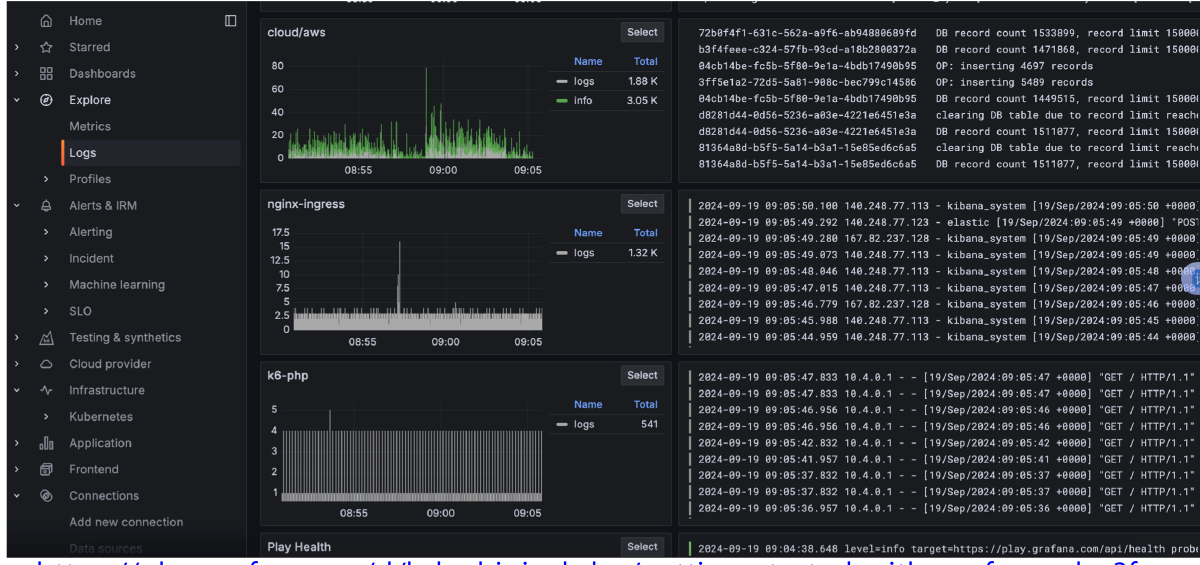
\includegraphics[width=\linewidth,height=.57\paperheight,keepaspectratio]{assets/week02-source-2025/grafana-behavior.png}
\column{.35\textwidth}
\begin{itemize}
  \item 指标聚合了某个时间窗口内的状态；
  \item 日志只记录被选择的局部事件；
  \item Trace 重建部分跨进程因果路径；
  \item 没有观测到不等于没有发生；
  \item 时间戳接近不等于存在因果关系。
\end{itemize}
\end{columns}
\smallnote{Grafana Play 可作为系统行为的直观入口。}
\end{frame}

\begin{frame}{模型、运行与观测：三个不同层次}
\begin{center}
\begin{tikzpicture}[node distance=13mm]
\node[draw=ADSBlue,fill=ADSLightBlue,rounded corners,minimum width=3.4cm,minimum height=.85cm] (model) {模型\scriptsize\quad 允许哪些执行};
\node[draw=ADSOrange,fill=ADSOrange!12,rounded corners,minimum width=3.4cm,minimum height=.85cm,right=of model] (run) {一次运行\scriptsize\quad 实际事件轨迹};
\node[draw=ADSGreen,fill=ADSGreen!10,rounded corners,minimum width=3.4cm,minimum height=.85cm,right=of run] (obs) {观测\scriptsize\quad 日志/指标/Trace};
\draw[ADSBlue,\arrow] (model)--(run);
\draw[ADSOrange,\arrow] (run)--(obs);
\draw[ADSGreen,\arrow,bend left=25] (obs) to node[below,font=\scriptsize]{验证/反驳假设} (model);
\end{tikzpicture}
\end{center}
\vfill
\begin{itemize}
  \item 模型用于证明所有允许执行都满足某种性质；
  \item 一次运行只是允许执行集合中的一个样本；
  \item 观测数据通常不完备，还受到采样、缓冲和时钟误差影响。
\end{itemize}
\end{frame}

\sectionframe{分布式程序与事件模型}{局部顺序与消息因果共同构成分布式执行的偏序。}

\begin{frame}{分布式程序：七项基本假设}
\small
\begin{enumerate}
  \item 程序由 $n$ 个异步进程 $p_1,p_2,\ldots,p_n$ 构成；
  \item 进程不共享全局内存，只通过消息通信；
  \item 进程不能瞬时读取一个共享全局时钟；
  \item 进程执行和消息传输都是异步的；
  \item 为便于讨论，假定每个进程运行在不同处理器上；
  \item $C_{ij}$ 表示从 $p_i$ 到 $p_j$ 的信道，$m_{ij}$ 表示相应消息；
  \item 消息传输延迟有限，但不可预测。
\end{enumerate}
\vfill
\callout{模型边界}{“有限但无已知上界”意味着消息最终到达，但超时不能证明接收方已经失败。}
\end{frame}

\begin{frame}{进程、信道与消息：执行的最小结构}
\begin{center}
\begin{tikzpicture}[node distance=21mm]
\nodebox{ADSBlue}{p1}{$p_i$\scriptsize\quad 局部状态};
\node[draw=ADSOrange,fill=ADSOrange!12,rounded corners,minimum width=3.4cm,minimum height=.8cm,right=of p1] (ch) {$C_{ij}$：在途消息集合/队列};
\nodebox[right=of ch]{ADSBlue}{p2}{$p_j$\scriptsize\quad 局部状态};
\draw[ADSOrange,\arrow] (p1)--node[above,font=\scriptsize]{$m_{ij}$} (ch);
\draw[ADSOrange,\arrow] (ch)--(p2);
\end{tikzpicture}
\end{center}
\vfill
\begin{itemize}
  \item 进程只直接修改自己的局部状态；
  \item 发送把信息写入信道，接收把信息从信道移入进程；
  \item 全局执行是多个局部执行与消息传输的组合。
\end{itemize}
\end{frame}

\begin{frame}{分布式执行：每个进程顺序执行原子动作}
\begin{itemize}
  \item 一个进程的执行由动作序列组成；
  \item 动作被建模为原子事件：不可分割、瞬时发生；
  \item $e_i^x$ 表示进程 $p_i$ 上的第 $x$ 个事件；
  \item 对消息 $m$，$send(m)$ 和 $rec(m)$ 分别表示发送与接收事件；
  \item 事件的发生会改变相关进程和信道的状态。
\end{itemize}
\vfill
\begin{center}
\begin{tikzpicture}[x=1.6cm]
\draw[->,ADSGray] (0,0)--(6,0);
\foreach \x/\lab in {1/$e_i^1$,2/$e_i^2$,3/$e_i^3$,4/$e_i^4$,5/$e_i^5$}{\fill[ADSBlue] (\x,0) circle (2pt) node[above,font=\scriptsize]{\lab};}
\end{tikzpicture}
\end{center}
\end{frame}

\begin{frame}{三类事件：internal、send、receive}
\begin{columns}[T,onlytextwidth]
\column{.31\textwidth}
\blocktitle{内部事件}
\begin{itemize}\item 发生在一个进程；\item 只改变该进程局部状态；\item 例如本地计算或定时器。\end{itemize}
\column{.31\textwidth}
\blocktitle{发送事件}
\begin{itemize}\item 改变发送进程状态；\item 将消息加入信道状态；\item 建立跨进程信息流。\end{itemize}
\column{.31\textwidth}
\blocktitle{接收事件}
\begin{itemize}\item 从信道取出消息；\item 改变接收进程状态；\item 依赖对应发送事件。\end{itemize}
\end{columns}
\end{frame}

\begin{frame}{事件如何改变进程与信道状态}
\scriptsize
\begin{tabularx}{\linewidth}{>{\bfseries}p{2.2cm}X X}
\toprule
事件 & 进程状态变化 & 信道状态变化 \\
\midrule
内部事件 $e_i^x$ & $p_i$ 的寄存器、栈、局部内存或应用状态变化 & 无直接变化 \\
发送 $send(m_{ij})$ & $p_i$ 的发送序号、缓存或协议状态变化 & $m_{ij}$ 进入 $C_{ij}$ \\
接收 $rec(m_{ij})$ & $p_j$ 消费消息并更新局部状态 & $m_{ij}$ 离开 $C_{ij}$ \\
\bottomrule
\end{tabularx}
\vfill
\callout{状态转移视角}{每个事件都是一个局部状态机转移；消息把一个状态机的输出变成另一个状态机的输入。}
\end{frame}

\begin{frame}{进程历史：局部事件具有全序}
\begin{itemize}
  \item 进程 $p_i$ 产生事件序列 $e_i^1,e_i^2,\ldots,e_i^x,e_i^{x+1},\ldots$；
  \item 其执行历史记为
  \[
    H_i=(h_i,\rightarrow_i),
  \]
  其中 $h_i$ 是 $p_i$ 产生的事件集合；
  \item $\rightarrow_i$ 按事件在 $p_i$ 上的发生顺序定义线性序；
  \item $e_i^x\rightarrow_i e_i^y$ 表示在同一进程上 $x<y$，因此前者因果先于后者。
\end{itemize}
\vfill
\smallnote{局部历史容易记录；困难在于如何组合不同进程的历史。}
\end{frame}

\begin{frame}{消息关系：发送因果先于对应接收}
\begin{center}
\begin{tikzpicture}[x=1.4cm,y=1.4cm]
\draw[->,ADSGray] (0,1)--(7,1) node[left,font=\scriptsize]{$p_i$};
\draw[->,ADSGray] (0,0)--(7,0) node[left,font=\scriptsize]{$p_j$};
\fill[ADSBlue] (2,1) circle (2.3pt) node[above,font=\scriptsize]{$send(m)$};
\fill[ADSBlue] (5,0) circle (2.3pt) node[below,font=\scriptsize]{$rec(m)$};
\draw[ADSOrange,\arrow,line width=1pt] (2,1)--(5,0);
\end{tikzpicture}
\end{center}
\vfill
\[
send(m)\rightarrow_{msg} rec(m)
\]
\begin{itemize}
  \item 消息携带的信息在发送之前存在，在接收之后才可能被接收方使用；
  \item $\rightarrow_{msg}$ 只连接同一消息的发送/接收事件；
  \item 它与进程内全序共同构成全局因果关系。
\end{itemize}
\end{frame}

\begin{frame}{时空图：把局部顺序与消息流画在一起}
\begin{itemize}
  \item 水平线表示进程随时间的推进；
  \item 点表示原子事件；
  \item 斜箭头表示消息传输；
  \item 左右位置用于表达图中的先后，不代表不同进程共享精确物理时钟；
  \item 若存在沿进程线向右和消息箭头组成的路径，则存在因果关系。
\end{itemize}
\vfill
\callout{读图规则}{只沿进程时间方向向右走，消息只能从发送端走向接收端。}
\end{frame}

\begin{frame}{分布式执行的时空图}
\begin{center}
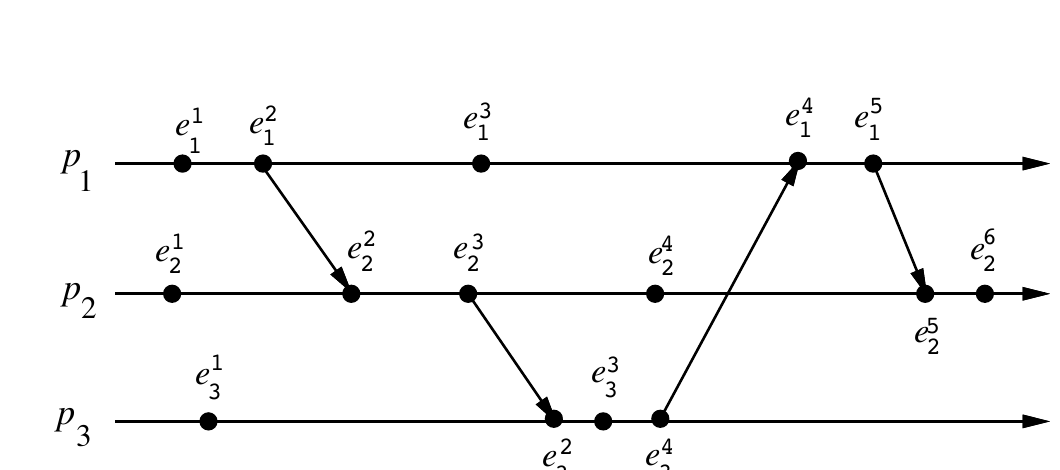
\includegraphics[width=.90\linewidth,height=.56\paperheight,keepaspectratio]{assets/week02-source-2025/execution-space-time.png}
\end{center}
\vfill
\smallnote{对 $p_1$ 而言：第二个事件是发送，第三个事件是内部事件，第四个事件是接收。}
\end{frame}

\begin{frame}{读图练习：哪些事件可能知道哪些信息？}
\begin{columns}[T,onlytextwidth]
\column{.54\textwidth}
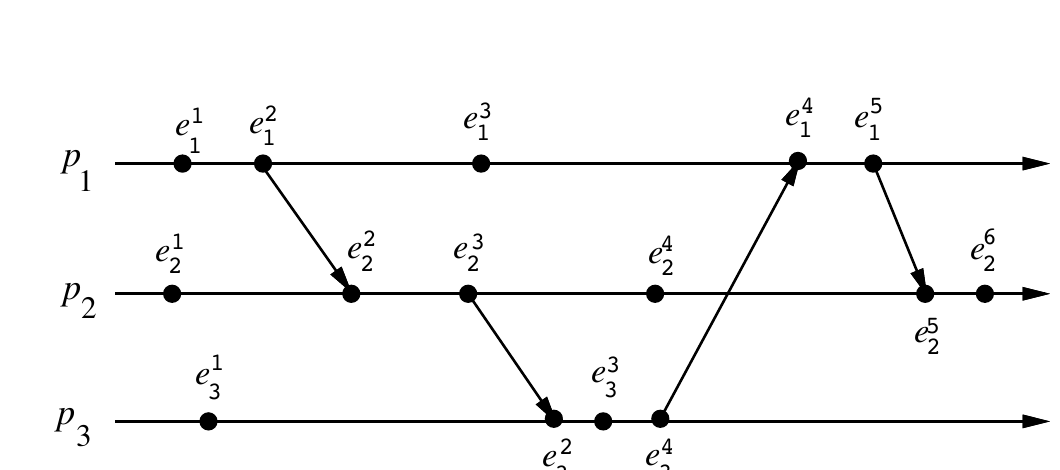
\includegraphics[width=\linewidth,height=.50\paperheight,keepaspectratio]{assets/week02-source-2025/execution-space-time.png}
\column{.40\textwidth}
\begin{enumerate}
  \item 找出 $e_1^1\rightarrow e_3^3$ 的一条路径；
  \item 判断 $e_1^3$ 与 $e_3^3$ 是否有因果关系；
  \item 找出图中最“知情”的事件；
  \item 改变消息延迟会不会改变局部程序顺序？
\end{enumerate}
\end{columns}
\vfill
\callout{课堂输出}{为每个判断写出路径证据，或说明双向都不存在路径。}
\end{frame}

\begin{frame}{因果先行关系：三条生成规则}
令 $H=\bigcup_i h_i$ 为执行中的所有事件。关系 $\rightarrow$ 是满足下列规则的最小传递关系：
\begin{enumerate}
  \item \key{进程顺序}：若 $i=j$ 且 $x<y$，则 $e_i^x\rightarrow e_j^y$；
  \item \key{消息顺序}：若 $e_i^x=send(m)$ 且 $e_j^y=rec(m)$，则 $e_i^x\rightarrow e_j^y$；
  \item \key{传递性}：若存在 $e_k^z$ 使 $e_i^x\rightarrow e_k^z$ 且 $e_k^z\rightarrow e_j^y$，则 $e_i^x\rightarrow e_j^y$。
\end{enumerate}
\vfill
\[
H=(H,\rightarrow)
\]
\smallnote{该关系是不可自反的偏序，也就是 Lamport 的 happened-before。}
\end{frame}

\begin{frame}{Happened-before：路径就是因果证据}
\begin{itemize}
  \item 若 $e_i\rightarrow e_j$，则 $e_j$ 直接或间接依赖于 $e_i$；
  \item 图上存在一条从 $e_i$ 到 $e_j$ 的有向路径；
  \item 进程线段必须沿时间增加方向，消息边必须沿发送到接收方向；
  \item $e_i$ 可用的信息有可能在 $e_j$ 处可访问；
  \item “有可能知道”不等于应用一定保存或使用了这些信息。
\end{itemize}
\vfill
\callout{知识视角}{因果偏序刻画信息传播的上限：没有因果路径，就没有基于该执行的信息来源。}
\end{frame}

\begin{frame}{信息流与“知道”：因果是可达性}
\begin{center}
\begin{tikzpicture}[node distance=13mm]
\node[draw=ADSBlue,fill=ADSLightBlue,rounded corners] (a) {$e_a$};
\node[draw=ADSOrange,fill=ADSOrange!12,rounded corners,right=of a] (b) {$e_b$};
\node[draw=ADSGreen,fill=ADSGreen!10,rounded corners,right=of b] (c) {$e_c$};
\draw[ADSBlue,\arrow] (a)--node[above,font=\scriptsize]{local/message} (b);
\draw[ADSOrange,\arrow] (b)--node[above,font=\scriptsize]{local/message} (c);
\end{tikzpicture}
\end{center}
\vfill
\begin{itemize}
  \item $e_a\rightarrow e_b\rightarrow e_c$，故 $e_a\rightarrow e_c$；
  \item 在执行模型中，$e_c$ 可能继承从 $e_a$ 传播的全部信息；
  \item 对应工程证据可以是上下文、版本号、请求 ID、向量时钟或 trace context；
  \item 没有显式传播元数据时，真实因果可能存在，但观测系统未必能恢复。
\end{itemize}
\end{frame}

\begin{frame}{非因果关系：不能把“未知”当作“并发”}
\begin{itemize}
  \item $e_i\not\rightarrow e_j$ 表示 $e_j$ 不直接或间接依赖 $e_i$；
  \item 此时 $e_j$ 不会因该执行中的 $e_i$ 获得信息；
  \item 但 $e_i\not\rightarrow e_j$ \orange{不能推出} $e_j\not\rightarrow e_i$；
  \item 若 $e_i\rightarrow e_j$，则必有 $e_j\not\rightarrow e_i$，否则形成因果环；
  \item 判断并发必须同时检查两个方向。
\end{itemize}
\vfill
\begin{center}\Large
$e_i\parallel e_j\quad\Longleftrightarrow\quad
e_i\not\rightarrow e_j\;\land\;e_j\not\rightarrow e_i$
\end{center}
\end{frame}

\begin{frame}{并发事件：偏序中互不可达的事件}
\begin{itemize}
  \item 两个事件互不因果影响时称为逻辑并发；
  \item 对任意两个不同事件，三种情况恰有一种成立：
  \[
    e_i\rightarrow e_j,\qquad e_j\rightarrow e_i,\qquad e_i\parallel e_j;
  \]
  \item 并发不是“同时发生”，而是执行结果不要求二者具有固定先后；
  \item 调度器、网络延迟变化后，逻辑并发事件可以交换物理发生顺序。
\end{itemize}
\vfill
\callout{算法意义}{并发事件之间的任意排序都必须被正确处理，除非协议显式建立顺序。}
\end{frame}

\begin{frame}{并发关系不具有传递性}
\begin{center}
\begin{tikzpicture}[node distance=18mm]
\node[draw=ADSBlue,fill=ADSLightBlue,rounded corners] (a) {$e_a$};
\node[draw=ADSOrange,fill=ADSOrange!12,rounded corners,right=of a] (b) {$e_b$};
\node[draw=ADSGreen,fill=ADSGreen!10,rounded corners,right=of b] (c) {$e_c$};
\draw[ADSGray,dashed,<->] (a)--node[above,font=\scriptsize]{$\parallel$} (b);
\draw[ADSGray,dashed,<->] (b)--node[above,font=\scriptsize]{$\parallel$} (c);
\draw[ADSBlue,\arrow,bend right=32] (a) to node[below,font=\scriptsize]{$\rightarrow$ 仍可能成立} (c);
\end{tikzpicture}
\end{center}
\vfill
\[
(e_a\parallel e_b)\land(e_b\parallel e_c)
\not\Rightarrow e_a\parallel e_c
\]
\begin{itemize}
  \item 并发是偏序的不可比关系，不是等价关系；
  \item 不能把一组两两局部并发的判断简单合并为“全都并发”。
\end{itemize}
\end{frame}

\begin{frame}{逻辑并发与物理并发}
\begin{columns}[T,onlytextwidth]
\column{.47\textwidth}
\blocktitle{逻辑并发}
\begin{itemize}
  \item 双向均无因果路径；
  \item 与处理器速度和消息延迟的具体数值无关；
  \item 是分布式算法分析的主要概念。
\end{itemize}
\column{.47\textwidth}
\blocktitle{物理并发}
\begin{itemize}
  \item 事件在同一物理时刻发生；
  \item 需要共享时间基准和足够精度；
  \item 物理不同时仍可能逻辑并发。
\end{itemize}
\end{columns}
\vfill
\callout{关键结论}{改变处理器速度或网络延迟可以让逻辑并发事件在物理时间上重合，但不改变计算结果中的因果偏序。}
\end{frame}

\begin{frame}{课堂互动：因果图的三色标注}
\begin{columns}[T,onlytextwidth]
\column{.55\textwidth}
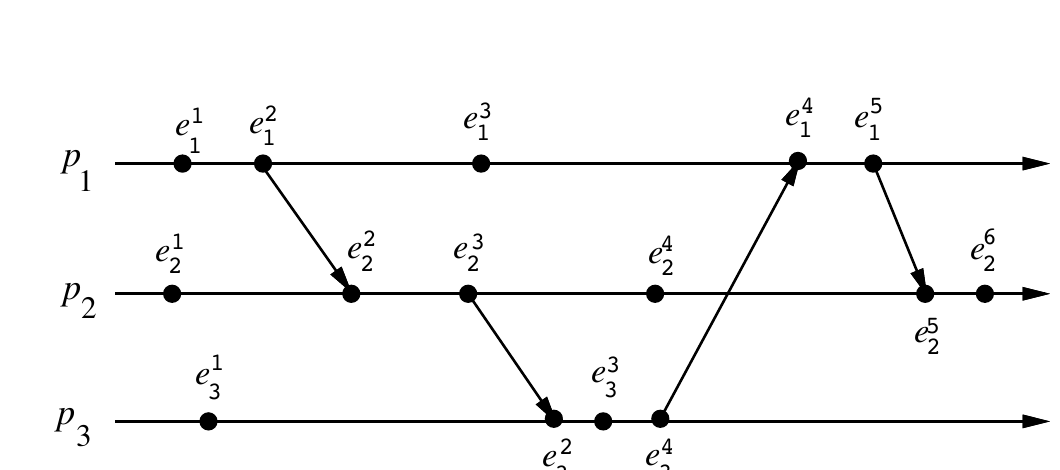
\includegraphics[width=\linewidth,height=.51\paperheight,keepaspectratio]{assets/week02-source-2025/execution-space-time.png}
\column{.39\textwidth}
\begin{enumerate}
  \item 选择一个目标事件；
  \item 蓝色标出它的 causal past；
  \item 橙色标出它的 causal future；
  \item 灰色标出与它并发的事件；
  \item 说明每种颜色的路径证据。
\end{enumerate}
\end{columns}
\vfill
\smallnote{输出：一张标注图 + 一条“并发不传递”的反例。}
\end{frame}

\sectionframe{通信网络与通信方式}{信道提供的顺序保证，会直接改变算法需要携带的控制信息。}

\begin{frame}{通信网络模型：FIFO、Non-FIFO、Causal}
\begin{columns}[T,onlytextwidth]
\column{.31\textwidth}\callout{FIFO}{同一发送方到同一接收方的信道保持发送顺序。}
\column{.31\textwidth}\callout{Non-FIFO}{信道像集合；消息可以按任意顺序被移除和交付。}
\column{.31\textwidth}\callout{Causal}{对同一目的地，所有因果相关消息按因果顺序交付。}
\end{columns}
\vfill
\callout{建模提醒}{“网络可靠”与“网络有序”是两个不同假设；可靠交付并不自动保证顺序。}
\end{frame}

\begin{frame}{FIFO 信道：每条信道是一条消息队列}
\begin{center}
\begin{tikzpicture}[node distance=7mm]
\nodebox{ADSBlue}{sender}{发送方 $p_i$};
\node[draw=ADSOrange,fill=ADSOrange!12,minimum width=1.2cm,minimum height=.75cm,right=of sender] (m1) {$m_1$};
\node[draw=ADSOrange,fill=ADSOrange!12,minimum width=1.2cm,minimum height=.75cm,right=of m1] (m2) {$m_2$};
\node[draw=ADSOrange,fill=ADSOrange!12,minimum width=1.2cm,minimum height=.75cm,right=of m2] (m3) {$m_3$};
\nodebox[right=of m3]{ADSBlue}{recv}{接收方 $p_j$};
\draw[ADSBlue,\arrow] (sender)--(m1);
\draw[ADSOrange,\arrow] (m1)--(m2);
\draw[ADSOrange,\arrow] (m2)--(m3);
\draw[ADSOrange,\arrow] (m3)--(recv);
\end{tikzpicture}
\end{center}
\vfill
\[
send_i(m_1)\rightarrow_i send_i(m_2)
\Rightarrow rec_j(m_1)\rightarrow_j rec_j(m_2)
\]
\smallnote{FIFO 只保证同一信道内的顺序，不保证来自不同发送方的消息之间存在顺序。}
\end{frame}

\begin{frame}{Non-FIFO 信道：到达与交付可以重排}
\begin{columns}[T,onlytextwidth]
\column{.48\textwidth}
\begin{tikzpicture}[x=1.1cm,y=.9cm]
\draw[->,ADSGray] (0,1)--(5.2,1) node[left,font=\scriptsize]{$p_i$};
\draw[->,ADSGray] (0,0)--(5.2,0) node[left,font=\scriptsize]{$p_j$};
\fill[ADSBlue] (1,1) circle (2pt) node[above,font=\scriptsize]{$m_1$};
\fill[ADSBlue] (2,1) circle (2pt) node[above,font=\scriptsize]{$m_2$};
\draw[ADSOrange,\arrow] (1,1)--(4,0);
\draw[ADSGreen,\arrow] (2,1)--(3,0);
\end{tikzpicture}
\column{.46\textwidth}
\begin{itemize}
  \item 后发送的 $m_2$ 可能先到达；
  \item 多路径、重传、并行处理都可能造成重排；
  \item 算法需使用序号、版本、去重表或重排缓冲区；
  \item TCP 字节流有序不代表应用层跨连接事件全局有序。
\end{itemize}
\end{columns}
\end{frame}

\begin{frame}{因果有序交付：保持消息之间的因果}
对发往同一目的进程 $p_j$ 的两条消息 $m_{ij}$ 与 $m_{kj}$，若
\[
send(m_{ij})\rightarrow send(m_{kj}),
\]
则因果有序系统保证
\[
rec(m_{ij})\rightarrow rec(m_{kj}).
\]
\vfill
\begin{itemize}
  \item 因果关系可以跨越不同发送方；
  \item 接收方不会先看到“回复”，后看到导致该回复的“请求/上下文”；
  \item 需要向量时间、依赖集合或等价控制信息；
  \item 内建因果有序可以简化上层分布式算法。
\end{itemize}
\end{frame}

\begin{frame}{三种顺序模型的关系}
\begin{center}
\begin{tikzpicture}
\draw[fill=ADSLightGray,draw=ADSGray] (0,0) ellipse (5.6cm and 2.1cm);
\draw[fill=ADSOrange!12,draw=ADSOrange] (0,0) ellipse (3.9cm and 1.5cm);
\draw[fill=ADSLightBlue,draw=ADSBlue] (0,0) ellipse (2.2cm and .9cm);
\node at (0,0) {Causal ordering};
\node at (0,-1.18) {FIFO};
\node at (0,-1.82) {Non-FIFO};
\end{tikzpicture}
\end{center}
\vfill
\[
\text{Causal ordering}\subset\text{FIFO}\subset\text{Non-FIFO}
\]
\smallnote{集合包含表示允许执行的集合：保证越强，允许的消息交付顺序越少。}
\end{frame}

\begin{frame}{顺序反例：FIFO 仍不足以保证跨发送方因果}
\begin{center}
\begin{tikzpicture}[x=1.2cm,y=.9cm]
\draw[->,ADSGray] (0,2)--(7,2) node[left,font=\scriptsize]{$p_1$};
\draw[->,ADSGray] (0,1)--(7,1) node[left,font=\scriptsize]{$p_2$};
\draw[->,ADSGray] (0,0)--(7,0) node[left,font=\scriptsize]{$p_3$};
\fill[ADSBlue] (1,2) circle (2pt) node[above,font=\scriptsize]{$send(m)$};
\fill[ADSBlue] (3,1) circle (2pt) node[above,font=\scriptsize]{$rec(m)$};
\fill[ADSOrange] (3.6,1) circle (2pt) node[above,font=\scriptsize]{$send(reply)$};
\fill[ADSOrange] (5,0) circle (2pt) node[below,font=\scriptsize]{$rec(reply)$};
\fill[ADSBlue] (6,0) circle (2pt) node[below,font=\scriptsize]{$rec(m)$};
\draw[ADSBlue,\arrow] (1,2)--(3,1);
\draw[ADSBlue,\arrow] (1,2)--(6,0);
\draw[ADSOrange,\arrow] (3.6,1)--(5,0);
\end{tikzpicture}
\end{center}
\vfill
\smallnote{两条信道各自都满足 FIFO，但 $p_3$ 先收到 reply，后收到其因果前驱 $m$；只有因果有序能排除该执行。}
\end{frame}

\begin{frame}{同步与异步进程通信模型}
\begin{columns}[T,onlytextwidth]
\column{.47\textwidth}
\blocktitle{同步通信}
\begin{itemize}
  \item 发送是阻塞式；
  \item 发送者等待接收者接受消息；
  \item 双方通过一次消息交换同步；
  \item 控制流简单，但容易产生等待链。
\end{itemize}
\column{.47\textwidth}
\blocktitle{异步通信}
\begin{itemize}
  \item 发送者不等待消息交付；
  \item 系统缓冲消息，在接收者就绪时交付；
  \item 可重叠计算和通信；
  \item 需要处理缓冲、背压和更高非确定性。
\end{itemize}
\end{columns}
\end{frame}

\begin{frame}{同步/异步通信：没有绝对优劣}
\scriptsize
\begin{tabularx}{\linewidth}{>{\bfseries}p{2.2cm}X X}
\toprule
维度 & 同步通信 & 异步通信 \\
\midrule
并行性 & 频繁阻塞，较低 & 消息在途时继续计算，较高 \\
缓冲管理 & 相对简单 & 突发发送可能溢出，需要背压 \\
算法设计 & 控制直观 & 非确定性更高，验证更困难 \\
性能风险 & 等待与死锁 & 排队、拥塞、内存增长 \\
实现重点 & 握手、超时、死锁避免 & 队列、流控、完成通知、资源回收 \\
\bottomrule
\end{tabularx}
\vfill
\callout{工程结论}{通信 API 的“非阻塞”只移动了等待位置，并没有消除完成、失败和资源生命周期问题。}
\end{frame}

\begin{frame}{工程映射：RPC、消息队列与 Actor}
\begin{columns}[T,onlytextwidth]
\column{.31\textwidth}
\blocktitle{RPC}
\begin{itemize}\item 表面同步调用；\item 超时后结果不确定；\item 重试可能重复执行。\end{itemize}
\column{.31\textwidth}
\blocktitle{消息队列}
\begin{itemize}\item 异步解耦；\item 需要消费确认和背压；\item 顺序范围由分区决定。\end{itemize}
\column{.31\textwidth}
\blocktitle{Actor / Ray}
\begin{itemize}\item 状态封装在 actor；\item 消息驱动执行；\item 调度和失败恢复由运行时协调。\end{itemize}
\end{columns}
\vfill
\callout{模型审查}{先问“顺序、可靠性、完成和故障语义是什么”，再选择通信库。}
\end{frame}

\sectionframe{全局状态与一致切面}{无法同时读取所有节点时，用不违反因果的状态组合替代“同一时刻快照”。}

\begin{frame}{分布式系统的全局状态}
\begin{center}\Large\color{ADSDarkBlue}
“进程局部状态与通信信道状态的集合”
\end{center}
\vfill
\begin{itemize}
  \item 进程状态包括寄存器、栈、局部内存及应用定义的状态；
  \item 信道状态是尚在传输中的消息集合；
  \item 内部事件只改变一个进程状态；
  \item 发送事件改变发送进程和相应信道；
  \item 接收事件改变接收进程和相应信道。
\end{itemize}
\end{frame}

\begin{frame}{局部状态记号}
\begin{itemize}
  \item $LS_i^x$ 表示 $p_i$ 在事件 $e_i^x$ 之后、$e_i^{x+1}$ 之前的状态；
  \item $LS_i^0$ 表示进程 $p_i$ 的初始状态；
  \item $LS_i^x$ 是 $p_i$ 执行到 $e_i^x$ 为止的全部局部事件的结果；
  \item 记 $send(m)\le LS_i^x$：发送事件已包含在该局部状态的过去；
  \item 记 $rec(m)\not\le LS_j^y$：对应接收事件尚未包含在接收方局部状态的过去。
\end{itemize}
\vfill
\begin{center}
\begin{tikzpicture}[x=1.3cm]
\draw[->,ADSGray] (0,0)--(7,0);
\foreach \x in {1,2,3,4,5,6}{\fill[ADSBlue] (\x,0) circle (2pt) node[above,font=\scriptsize]{$e_i^{\x}$};}
\draw[ADSOrange,very thick] (0.15,-.3)--(3.5,-.3) node[midway,below,font=\scriptsize]{$LS_i^3$ 包含的过去};
\end{tikzpicture}
\end{center}
\end{frame}

\begin{frame}{信道状态：已发送但尚未接收的消息}
信道 $C_{ij}$ 在发送方状态 $LS_i^x$ 与接收方状态 $LS_j^y$ 下的状态为
\[
SC_{ij}^{x,y}=\{m_{ij}\mid
send(m_{ij})\le LS_i^x\;\land\;
rec(m_{ij})\not\le LS_j^y\}.
\]
\vfill
\begin{itemize}
  \item 消息的发送已发生，因此它属于全局状态；
  \item 消息的接收尚未发生，因此它仍位于信道中；
  \item 信道状态依赖两端选取的局部状态；
  \item 同一物理信道在不同切面上可以包含不同的在途消息。
\end{itemize}
\end{frame}

\begin{frame}{全局状态：局部状态与信道状态的组合}
\[
GS=\{LS_1^{x_1},\ldots,LS_n^{x_n},
SC_{12}^{x_1,x_2},\ldots,SC_{ij}^{x_i,x_j},\ldots\}.
\]
\vfill
\begin{itemize}
  \item 若所有组件状态在同一物理时刻记录，组合自然有意义；
  \item 但不存在可被所有进程瞬时读取的全局时钟；
  \item 物理时钟也不可能完美同步；
  \item 因此我们需要比“同一时刻”更弱、但仍有意义的条件：\key{一致性}。
\end{itemize}
\end{frame}

\begin{frame}{一致全局状态：结果不能先于原因出现}
\begin{center}\Large
每个被记录为“已接收”的消息，也必须被记录为“已发送”。
\end{center}
\vfill
\begin{itemize}
  \item 一致状态不违反 happened-before；
  \item 不能出现接收事件位于过去，而对应发送事件位于未来；
  \item 一个消息可以被记录为已发送但未接收，此时它属于信道状态；
  \item 不一致全局状态不是系统真实可能到达的状态，因此不能用于正确推理。
\end{itemize}
\vfill
\callout{直觉}{可以看到“原因发生、结果尚未发生”，不能看到“结果发生、原因尚未发生”。}
\end{frame}

\begin{frame}{一致性的形式化条件：过去对因果前驱闭包}
令 $PAST(GS)$ 表示全局状态中已经记录的事件集合，则
\[
GS\text{ 一致}
\quad\Longleftrightarrow\quad
\forall e\in PAST(GS),\; e'\rightarrow e
\Rightarrow e'\in PAST(GS).
\]
\vfill
对每条消息 $m_{ij}$：
\begin{itemize}
  \item 若 $rec(m_{ij})$ 已包含在 $LS_j^{x_j}$ 中，则 $send(m_{ij})$ 必须包含在 $LS_i^{x_i}$ 中；
  \item 若只包含发送而不包含接收，则 $m_{ij}$ 必须出现在 $SC_{ij}^{x_i,x_j}$ 中；
  \item 该条件也称为因果向下闭包（downward closed）。
\end{itemize}
\end{frame}

\begin{frame}{全局状态示例：四个进程的执行}
\begin{center}
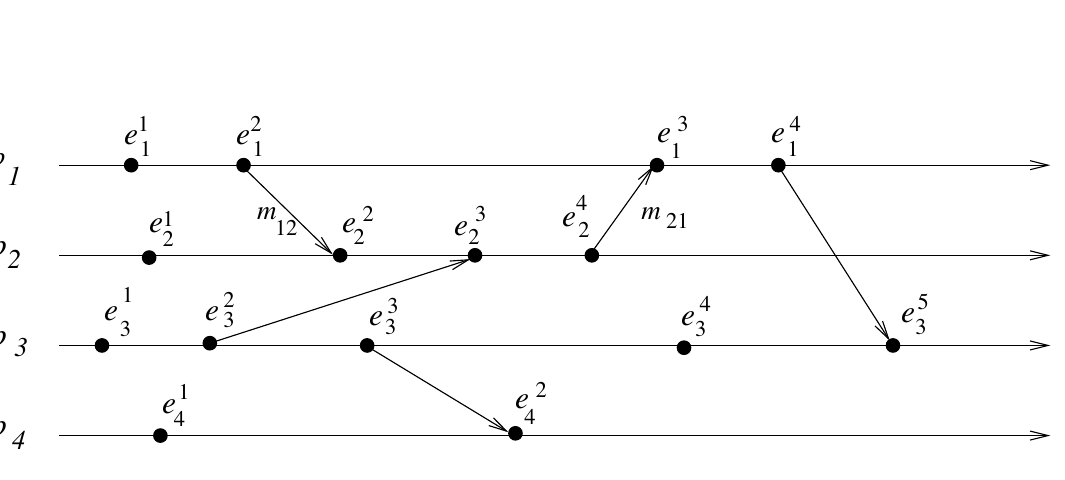
\includegraphics[width=.92\linewidth,height=.57\paperheight,keepaspectratio]{assets/week02-source-2025/global-state-example.png}
\end{center}
\vfill
\smallnote{下面比较两个局部状态组合：一个包含“无发送的接收”，另一个只包含合法在途消息。}
\end{frame}

\begin{frame}{$GS_1$：包含结果但遗漏原因，因此不一致}
\[
GS_1=\{LS_1^1,LS_2^3,LS_3^3,LS_4^2\}.
\]
\begin{itemize}
  \item $p_2$ 的状态已经记录接收消息 $m_{12}$；
  \item 但 $p_1$ 的状态尚未记录 $m_{12}$ 的发送；
  \item 因此 $rec(m_{12})\in PAST(GS_1)$，而 $send(m_{12})\notin PAST(GS_1)$；
  \item 该切面从消息箭头的未来侧穿到过去侧，违反因果闭包。
\end{itemize}
\vfill
\begin{center}\Large\color{ADSOrange}\bfseries $GS_1$ 不一致\end{center}
\end{frame}

\begin{frame}{$GS_2$：发送已发生，接收尚未发生}
\[
GS_2=\{LS_1^2,LS_2^4,LS_3^4,LS_4^2\}.
\]
\begin{itemize}
  \item 所有已记录的接收事件都有对应发送事件；
  \item 除 $C_{21}$ 外，其余信道为空；
  \item 消息 $m_{21}$ 已由 $p_2$ 发送，但尚未被 $p_1$ 接收；
  \item 因而 $m_{21}\in SC_{21}$，表示一个合法在途消息。
\end{itemize}
\vfill
\begin{center}\Large\color{ADSGreen}\bfseries $GS_2$ 一致\end{center}
\end{frame}

\begin{frame}{Cut：在每条进程线上选择一个局部状态}
\begin{itemize}
  \item Cut 是连接每条进程线上任意一点的锯齿线；
  \item 它把执行中的事件分为 $PAST(C)$ 与 $FUTURE(C)$；
  \item Cut 左侧事件属于过去，右侧事件属于未来；
  \item 每个 cut 对应一个全局状态；
  \item 每个全局状态也可以画成时空图上的一个 cut。
\end{itemize}
\vfill
\callout{图形优势}{判断一致性可以转化为检查消息箭头如何穿越切面。}
\end{frame}

\begin{frame}{两个切面：$C_1$ 与 $C_2$}
\begin{center}
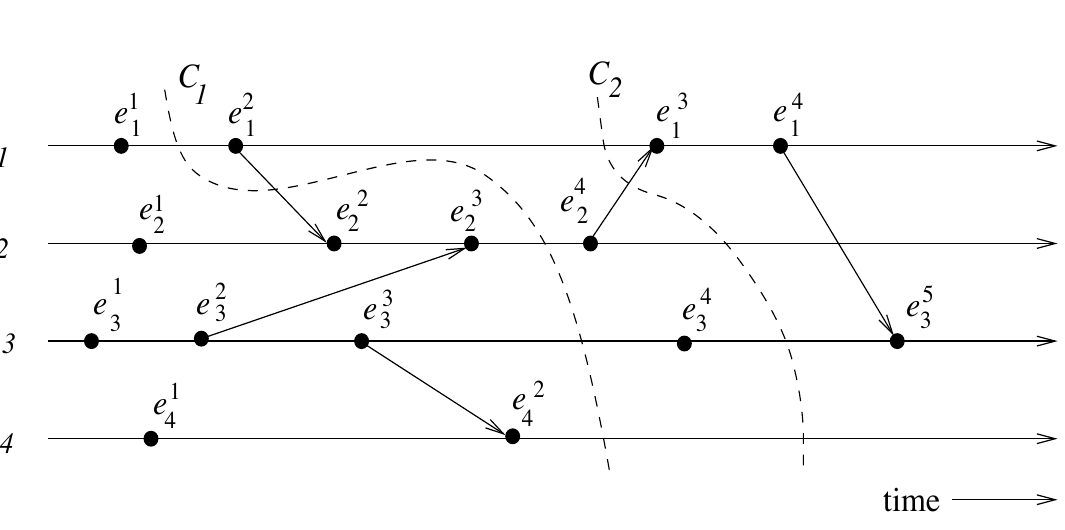
\includegraphics[width=.91\linewidth,height=.59\paperheight,keepaspectratio]{assets/week02-source-2025/cuts-example.png}
\end{center}
\smallnote{$C_1$ 有消息从未来穿向过去；$C_2$ 只允许消息从过去穿向未来。}
\end{frame}

\begin{frame}{一致切面：接收在过去，则发送也在过去}
\begin{itemize}
  \item 对任何消息，若接收事件位于 $PAST(C)$，发送事件也必须位于 $PAST(C)$；
  \item 所有从过去穿向未来的消息都是该全局状态中的在途消息；
  \item 一致切面对应一个系统可能经历的全局状态；
  \item 图中的 $C_2$ 是一致切面。
\end{itemize}
\vfill
\begin{center}
\begin{tikzpicture}[x=1.2cm,y=1cm]
\draw[->,ADSGray] (0,1)--(6,1);
\draw[->,ADSGray] (0,0)--(6,0);
\draw[ADSBlue,dashed,very thick] (3,-.25)--(3,1.25);
\draw[ADSOrange,\arrow] (2,1)--(4,0);
\node[font=\scriptsize] at (3.7,.75) {过去 $\rightarrow$ 未来：在途消息};
\end{tikzpicture}
\end{center}
\end{frame}

\begin{frame}{不一致切面：消息从未来穿向过去}
\begin{center}
\begin{tikzpicture}[x=1.2cm,y=1cm]
\draw[->,ADSGray] (0,1)--(6,1);
\draw[->,ADSGray] (0,0)--(6,0);
\draw[ADSBlue,dashed,very thick] (2.5,1.25)--(3.6,-.25);
\draw[ADSOrange,\arrow] (4,1)--(2,0);
\node[font=\scriptsize,ADSOrange] at (3.9,.25) {未来 $\rightarrow$ 过去};
\end{tikzpicture}
\end{center}
\vfill
\begin{itemize}
  \item 接收事件在切面过去侧；
  \item 对应发送事件却在未来侧；
  \item 组合状态包含一个没有原因的结果；
  \item 图中的 $C_1$ 就是不一致切面。
\end{itemize}
\end{frame}

\begin{frame}{穿越切面的消息如何解释？}
\scriptsize
\begin{tabularx}{\linewidth}{>{\bfseries}p{3.1cm}X X}
\toprule
发送/接收相对 cut & 含义 & 一致性 \\
\midrule
发送在过去，接收在过去 & 消息已被接收，不属于信道状态 & 合法 \\
发送在过去，接收在未来 & 消息在途，属于信道状态 & 合法 \\
发送在未来，接收在未来 & 消息尚未产生 & 合法 \\
发送在未来，接收在过去 & 结果先于原因 & 不合法 \\
\bottomrule
\end{tabularx}
\vfill
\callout{算法衔接}{第 4 周的快照算法，本质上是在异步执行中构造一个一致切面并记录在途消息。}
\end{frame}

\begin{frame}{课堂互动：银行转账切面}
\begin{columns}[T,onlytextwidth]
\column{.48\textwidth}
\blocktitle{场景}
\begin{itemize}
  \item 账户 A 扣款 100；
  \item 转账消息在信道中；
  \item 账户 B 随后入账 100；
  \item 目标：计算系统总余额。
\end{itemize}
\column{.48\textwidth}
\blocktitle{任务}
\begin{enumerate}
  \item 画出进程线与消息；
  \item 画一个一致 cut；
  \item 画一个不一致 cut；
  \item 说明在途消息如何计入总额。
\end{enumerate}
\end{columns}
\vfill
\smallnote{关键：扣款已记录、入账未记录时，信道状态必须包含 100。}
\end{frame}

\sectionframe{事件的过去锥与未来锥}{以一个事件为中心，划分可能影响它、受它影响和与它并发的事件。}

\begin{frame}{Past cone：可能影响目标事件的全部事件}
对计算 $(H,\rightarrow)$ 中的目标事件 $e_j$：
\[
Past(e_j)=\{e_i\in H\mid e_i\rightarrow e_j\}.
\]
\vfill
\begin{itemize}
  \item $e_j$ 只能受到其因果过去中事件的影响；
  \item $Past(e_j)$ 包含同一进程的历史和通过消息传播而来的历史；
  \item 若 $e_i\notin Past(e_j)$，则 $e_j$ 不可能通过该执行获得 $e_i$ 的信息；
  \item Past cone 是因果偏序中目标事件的下闭包。
\end{itemize}
\end{frame}

\begin{frame}{因果过去与因果未来的几何直觉}
\begin{center}
\begin{tikzpicture}[font=\small,>=Latex,scale=.82,transform shape]
  \fill[ADSBlue!9] (-6,-2.3)--(-2.7,-2.3)--(0,0)--(-2.7,2.3)--(-6,2.3)--cycle;
  \fill[ADSOrange!12] (6,-2.3)--(2.7,-2.3)--(0,0)--(2.7,2.3)--(6,2.3)--cycle;
  \draw[ADSGray] (-6,0)--(6,0);
  \draw[ADSGray] (-2.7,-2.3)--(0,0)--(-2.7,2.3);
  \draw[ADSGray] (2.7,-2.3)--(0,0)--(2.7,2.3);
  \fill[ADSBlue] (0,0) circle (2.5pt) node[below=2mm] {目标事件 $e_j$};
  \node[text=ADSBlue,font=\bfseries] at (-4,0) {因果过去};
  \node[text=ADSOrange,font=\bfseries] at (4,0) {因果未来};
  \fill[ADSBlue] (-2.7,0) circle (2pt) node[above=2mm,align=center] {进程 $i$ 上\\最近的因果前驱};
  \fill[ADSOrange] (2.7,0) circle (2pt) node[above=2mm,align=center] {进程 $i$ 上\\最早的因果后继};
  \node[text=ADSGray,align=center] at (0,-1.55) {锥体之外的事件\\与 $e_j$ 并发};
\end{tikzpicture}
\end{center}
\smallnote{蓝色区域表示因果过去，橙色区域表示因果未来；两者之外的事件与 $e_j$ 并发。}
\end{frame}

\begin{frame}{每个进程上的最近因果前驱}
定义
\[
Past_i(e_j)=Past(e_j)\cap h_i.
\]
由于 $p_i$ 上的事件全序，$Past_i(e_j)$ 也全序。其最大元素
\[
max(Past_i(e_j))
\]
是进程 $p_i$ 上影响 $e_j$ 的最新事件。
\vfill
\begin{itemize}
  \item 它概括目标事件从进程 $p_i$ 最多可能知道到哪里；
  \item 若不存在来自 $p_i$ 的因果信息，则该分量位于初始状态；
  \item 向量时钟的每个分量正是这种“最新已知进度”的编码。
\end{itemize}
\end{frame}

\begin{frame}{Past cone 的表面：每个进程一个最大事件}
\[
MaxPast(e_j)=\bigcup_i\{max(Past_i(e_j))\}.
\]
\begin{itemize}
  \item $MaxPast(e_j)$ 包含每个进程上影响 $e_j$ 的最新事件；
  \item 它构成 $e_j$ 过去锥的“表面”；
  \item 表面左侧是确定的因果过去；
  \item 表面之后的事件不一定影响 $e_j$；
  \item 用 $n$ 个分量即可压缩表达可能包含大量事件的过去集合。
\end{itemize}
\vfill
\callout{课程衔接}{第 3 周的向量时钟会把 $MaxPast$ 转化为可随消息传播的整数向量。}
\end{frame}

\begin{frame}{Future cone：受目标事件因果影响的事件}
\[
Future(e_j)=\{e_i\in H\mid e_j\rightarrow e_i\}.
\]
\begin{itemize}
  \item Future cone 包含所有直接或间接受 $e_j$ 影响的事件；
  \item 它是偏序中目标事件的上闭包；
  \item 一个故障、配置更新或权限变化的未来锥表示其潜在影响范围；
  \item 工程中的 blast radius 可以视为 future cone 的可观测近似。
\end{itemize}
\end{frame}

\begin{frame}{Future cone 的表面：每个进程的首个受影响事件}
定义
\[
Future_i(e_j)=Future(e_j)\cap h_i,
\]
并令 $min(Future_i(e_j))$ 为 $p_i$ 上第一个受 $e_j$ 影响的事件。则
\[
MinFuture(e_j)=\bigcup_i\{min(Future_i(e_j))\}.
\]
\begin{itemize}
  \item 它构成未来锥的表面；
  \item 表面之后的事件都可能继承 $e_j$ 的影响；
  \item 表面到达各进程的时间取决于消息路径与调度。
\end{itemize}
\end{frame}

\begin{frame}{并发区域：既不在过去，也不在未来}
\[
Concurrent(e_j)=H-Past(e_j)-Future(e_j)-\{e_j\}.
\]
\begin{itemize}
  \item 在每个进程上，位于 $max(Past_i(e_j))$ 之后、$min(Future_i(e_j))$ 之前的事件与 $e_j$ 并发；
  \item 这些事件既不能影响 $e_j$，也不受 $e_j$ 影响；
  \item 物理时间上它们可能早于、晚于或同时于 $e_j$；
  \item 任何强制排序都需要额外通信或共享同步机制。
\end{itemize}
\end{frame}

\begin{frame}{从因果锥到向量时间}
\begin{center}
\begin{tikzpicture}[node distance=13mm]
\node[draw=ADSBlue,fill=ADSLightBlue,rounded corners,minimum width=3cm,minimum height=.8cm] (past) {Past cone};
\node[draw=ADSOrange,fill=ADSOrange!12,rounded corners,minimum width=3cm,minimum height=.8cm,right=of past] (surface) {MaxPast 表面};
\node[draw=ADSGreen,fill=ADSGreen!10,rounded corners,minimum width=3cm,minimum height=.8cm,right=of surface] (vector) {向量时间};
\draw[ADSBlue,\arrow] (past)--node[above,font=\scriptsize]{每进程取最大事件} (surface);
\draw[ADSOrange,\arrow] (surface)--node[above,font=\scriptsize]{编码为计数器} (vector);
\end{tikzpicture}
\end{center}
\vfill
\begin{itemize}
  \item 事件集合可能很大，但表面只需每个进程一个位置；
  \item 向量时间通过比较分量判断因果与并发；
  \item 这是下一讲“逻辑时间”的概念起点。
\end{itemize}
\end{frame}

\sectionframe{模型选择与工程映射}{真实系统通常叠加时间、通信、故障、状态和观测模型。}

\begin{frame}{时间模型：同步、异步与部分同步}
\scriptsize
\begin{tabularx}{\linewidth}{>{\bfseries}p{2.3cm}X X X}
\toprule
 & 同步 & 异步 & 部分同步 \\
\midrule
进程速度 & 已知上下界 & 无已知上界 & 最终或在区间内有界 \\
消息延迟 & 已知上界 & 有限但不可预测 & 最终存在上界或上界未知 \\
超时含义 & 可作为故障证据 & 只能表示“尚未观察到” & 稳定期后可用于推进 \\
典型用途 & 轮次算法 & 不可能性与最弱假设 & 共识与工程系统 \\
\bottomrule
\end{tabularx}
\vfill
\smallnote{同一个系统可以在不同时间尺度或稳定阶段使用不同模型。}
\end{frame}

\begin{frame}{故障模型：算法究竟承诺处理什么？}
\begin{columns}[T,onlytextwidth]
\column{.23\textwidth}\callout{Crash}{进程停止，不再执行。}
\column{.23\textwidth}\callout{Omission}{发送、接收或信道丢失动作。}
\column{.23\textwidth}\callout{Timing}{行为正确但违反时间约束。}
\column{.23\textwidth}\callout{Byzantine}{节点可以任意偏离协议。}
\end{columns}
\vfill
\begin{itemize}
  \item 故障模型越强，协议通常需要更多副本、通信和验证；
  \item “慢节点”在异步模型中与“崩溃节点”不可立即区分；
  \item 安全性常要求始终成立，活性可能依赖最终同步或故障检测器。
\end{itemize}
\end{frame}

\begin{frame}{安全性与活性：模型中的两类性质}
\begin{columns}[T,onlytextwidth]
\column{.47\textwidth}
\blocktitle{Safety}
\begin{itemize}
  \item “坏事永远不发生”；
  \item 可由有限反例前缀证伪；
  \item 如：不会同时存在两个合法领导者。
\end{itemize}
\column{.47\textwidth}
\blocktitle{Liveness}
\begin{itemize}
  \item “好事最终发生”；
  \item 依赖调度公平、消息最终到达等假设；
  \item 如：请求最终得到响应或明确失败。
\end{itemize}
\end{columns}
\vfill
\callout{评审方法}{每个协议至少写出一条安全性、一条活性和它们依赖的模型假设。}
\end{frame}

\begin{frame}{状态机视角：把执行定义为状态与事件轨迹}
\begin{center}
\begin{tikzpicture}[node distance=9mm]
\node[draw=ADSBlue,fill=ADSLightBlue,rounded corners] (s0) {$S_0$};
\node[draw=ADSOrange,fill=ADSOrange!12,rounded corners,right=of s0] (s1) {$S_1$};
\node[draw=ADSGreen,fill=ADSGreen!10,rounded corners,right=of s1] (s2) {$S_2$};
\node[draw=ADSGray,fill=ADSLightGray,rounded corners,right=of s2] (s3) {$S_3$};
\draw[ADSBlue,\arrow] (s0)--node[above,font=\scriptsize]{$e_1$} (s1);
\draw[ADSOrange,\arrow] (s1)--node[above,font=\scriptsize]{$e_2$} (s2);
\draw[ADSGreen,\arrow] (s2)--node[above,font=\scriptsize]{$e_3$} (s3);
\end{tikzpicture}
\end{center}
\vfill
\begin{itemize}
  \item 状态定义系统此刻保存的信息；
  \item 事件定义合法状态转移；
  \item 执行是状态/事件组成的轨迹；
  \item 安全性限制可达状态，活性限制无限轨迹；
  \item I/O Automata、TLA+ 和状态机复制都建立在该视角上。
\end{itemize}
\end{frame}

\begin{frame}{分布式系统的可观测性边界}
\begin{center}
\begin{tikzpicture}[node distance=9mm]
\node[draw=ADSBlue,fill=ADSLightBlue,rounded corners] (real) {真实事件};
\node[draw=ADSOrange,fill=ADSOrange!12,rounded corners,right=of real] (instrument) {插桩/采样};
\node[draw=ADSGreen,fill=ADSGreen!10,rounded corners,right=of instrument] (transport) {异步传输};
\node[draw=ADSGray,fill=ADSLightGray,rounded corners,right=of transport] (view) {监控视图};
\draw[ADSBlue,\arrow] (real)--(instrument);
\draw[ADSOrange,\arrow] (instrument)--(transport);
\draw[ADSGreen,\arrow] (transport)--(view);
\end{tikzpicture}
\end{center}
\vfill
\begin{itemize}
  \item 日志可能丢失、延迟或乱序；
  \item 指标聚合会丢失单个事件及因果路径；
  \item Trace 只覆盖被传播上下文的请求；
  \item 监控界面本身也是一个异步分布式系统；
  \item 因此诊断结论必须说明观测模型与缺失数据。
\end{itemize}
\end{frame}

\begin{frame}{工程映射：Ray 中的进程、事件、消息与状态}
\begin{columns}[T,onlytextwidth]
\column{.48\textwidth}
\blocktitle{模型对象}
\begin{itemize}
  \item 进程：Driver、Worker、Actor、Scheduler；
  \item 消息：任务提交、对象引用、心跳与租约；
  \item 状态：Object Store、任务表、Actor 状态；
  \item 事件：调度、执行、完成、失败和重试。
\end{itemize}
\column{.48\textwidth}
\blocktitle{模型问题}
\begin{itemize}
  \item 对象创建与消费是否存在因果路径？
  \item Worker 超时表示慢还是崩溃？
  \item 重试如何避免重复副作用？
  \item 控制面看到的状态是否构成一致切面？
\end{itemize}
\end{columns}
\end{frame}

\begin{frame}{模型选择清单}
\scriptsize
\begin{tabularx}{\linewidth}{>{\bfseries}p{2.3cm}X}
\toprule
进程/对象 & 谁拥有状态？节点、进程、线程、Actor 还是服务？\\
通信 & 可靠性、顺序、重复、缓冲、背压和完成语义是什么？\\
时间 & 延迟是否有上界？超时可以证明什么？\\
故障 & 处理 Crash、Omission、Timing 还是 Byzantine？最多多少故障？\\
状态 & 哪些状态属于进程，哪些消息仍在信道中？\\
一致性 & 需要同时切面、因果一致，还是更弱的应用语义？\\
观测 & 哪些事件被记录？时钟误差、采样和丢失如何影响结论？\\
性质 & 安全性、活性与复杂度分别是什么？\\
\bottomrule
\end{tabularx}
\end{frame}

\begin{frame}{本讲总结：从局部事件推理全局行为}
\begin{center}
\begin{tikzpicture}[node distance=8mm]
\nodebox{ADSBlue}{local}{局部全序};
\nodebox[right=of local]{ADSOrange}{msg}{消息因果};
\nodebox[right=of msg]{ADSGreen}{partial}{全局偏序};
\nodebox[right=of partial]{ADSGray}{cut}{一致切面};
\draw[ADSBlue,\arrow] (local)--(msg);
\draw[ADSOrange,\arrow] (msg)--(partial);
\draw[ADSGreen,\arrow] (partial)--(cut);
\end{tikzpicture}
\end{center}
\vfill
\begin{itemize}
  \item 进程内顺序与消息边生成 happened-before；
  \item 双向无因果路径的事件逻辑并发；
  \item 通信网络可提供 Non-FIFO、FIFO 或因果有序保证；
  \item 全局状态由局部状态与信道状态组成；
  \item 一致 cut 不包含“无原因的结果”；
  \item Past/Future cone 为逻辑时钟和影响分析奠定基础。
\end{itemize}
\end{frame}

\begin{frame}{课堂互动：为真实系统写一份模型合同}
\begin{columns}[T,onlytextwidth]
\column{.48\textwidth}
\blocktitle{选择一个系统}
\begin{itemize}
  \item Ray 训练作业；
  \item Kafka 消息流；
  \item Kubernetes 控制器；
  \item 微服务请求链；
  \item 大模型推理集群。
\end{itemize}
\column{.48\textwidth}
\blocktitle{模型合同必须包含}
\begin{enumerate}
  \item 进程、信道、事件和状态；
  \item 时间、通信和故障假设；
  \item 一条安全性与一条活性；
  \item 一种可观测证据；
  \item 一个会使证明失效的反例。
\end{enumerate}
\end{columns}
\end{frame}

\begin{frame}{模型扩展：不要把不同故障假设混成一个系统}
\small
\begin{tabularx}{\linewidth}{>{\bfseries}p{3.0cm}XX}
\toprule
基础异步模型 & 消息最终到达，但没有已知延迟上界；适合定义 happened-before、cut 和快照。 & 超时只能说明“尚未观察到”，不能直接证明崩溃。 \\
Crash/Omission 扩展 & 进程可能停止，或消息可能丢失；需要重试、故障检测器或多数派。 & 需要明确“丢失一次”与“永久失联”是否可区分。 \\
Byzantine 扩展 & 节点可以发送矛盾或伪造信息；通常还需要认证、签名和更强副本数条件。 & 不能把 Crash 模型下的安全性直接升级为 Byzantine 安全性。 \\
\bottomrule
\end{tabularx}
\vfill
\callout{审题规则}{每个定理、复杂度和“最终会发生”都必须绑定到一个明确的模型；换模型以后，结论要重新证明。}
\end{frame}

\begin{frame}[plain]
\begin{tikzpicture}[remember picture,overlay]
  \fill[ADSBlue] (current page.north west) rectangle (current page.south east);
  \fill[ADSOrange] (current page.south west) rectangle ([yshift=2mm]current page.south east);
  \node[align=center] at (current page.center) {\fontsize{38}{45}\selectfont\color{white}\bfseries 谢谢\\[5mm]
  \large\color{white!80}下一讲：逻辑时间};
\end{tikzpicture}
\end{frame}

\end{document}
